$K$D-Tree is a space partitioning structure that can be used to organise data points in $k$ dimensional space. We have fixed our dimensions of data points to $2$-dimensions and their values are stored as a scalar. In our implementation, $K$D-Tree is a binary tree with every node having data points partitioned in $2$-dimensional space. A $K$D-Tree is a binary tree since each node has two children and when the keys are multidimensional each node is partitioned at split axis based on the depth of the tree and the dimension of the key which in turn determines the number of split axis the tree will have. For example for a $3$-dimensional space the first split axis is x-coordinate and then at the next level it will be y-coordinate and lastly z-coordinate.

% The following is not strictly definitions, but more like properties.
\subsubsection{Properties}

\begin{figure}[htp]
    \centering
    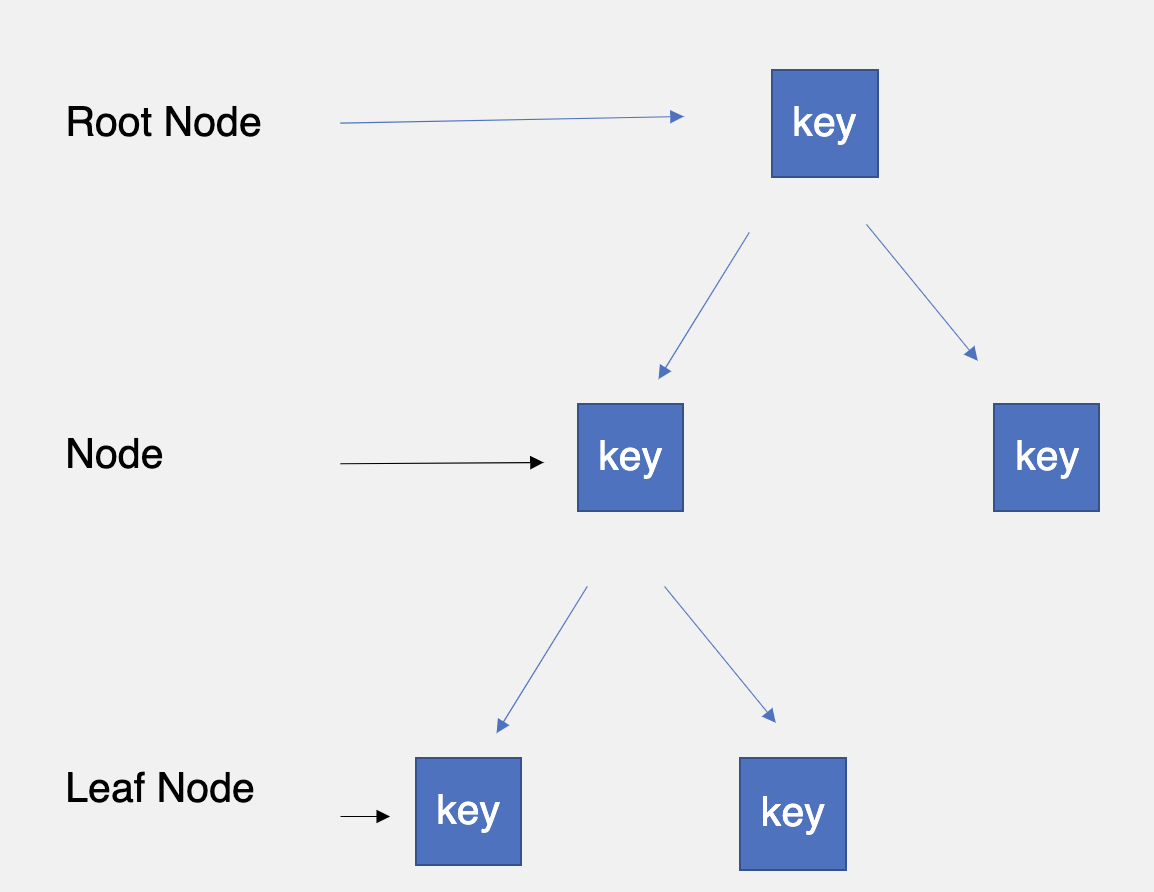
\includegraphics[width=0.4\textwidth]{graphs/KD-Tree.png}
    \caption{$K$D-Tree}
    \label{fig:$K$D-Tree}
\end{figure}

\begin{enumerate}
    \item\textbf{Node}: Node of a $K$D-Tree is essentially a $2$-dimensional data point. It can be k-dimensional for $K$D-Tree. Node is called a Root Node when it is at the top level as can be seen in Fig. \ref{fig:$K$D-Tree} and does not have a parent. A node is called a Leaf Node when it has no children and is at the bottom level. 

    \item\textbf{Levels}: Nodes are at the same level when they have the same distance from root. Hence, a level increases as the distance of the nodes increase from root. In the \ref{fig:$K$D-Tree} we can see the key at root is at level $1$ and then we have level $2$ and level $3$. 
    \item\textbf{Dimensions}: Every $K$D-Tree can be structured in such a way that the data points are divided into $k$-dimensions. Each node is recursively cut into as many dimensions as is mentioned in the dimensions. In our case the data points are $2$-dimensional and hence the space is divided into $2$-dimensions alternatively until a leaf is reached.
\end{enumerate}
    
\begin{algorithm}[H]
    \SetAlgoLined
    \SetKwInOut{Input}{Input}
    \SetKwInOut{Output}{Output}
    \Input{pointList; Keys=[$(x,y);x \in \mathbb{R};y \in \mathbb{R}$], dimension = 2,  split\_axis; 0 or 1}
    \Output{$K$D-Tree}
    \For{$i\gets0$ \KwTo $len(pointList)$}{
    \texttt{$int$ split\_axis := split\_axis mod $dimension$} // Select the split\_axis based on depth\\
    \texttt{Sort point list and choose median}\\
    \texttt{Create node at median}\\
    \texttt{node.leftChild := kdtree(points in pointList before median, split\_axis+1); //SubTree Creation \\ 
    node.rightChild := kdtree(points in pointList after median, split\_axis+1);}\\
    return node
     \caption{Construction Algorithm for $K$D-Tree}
     \label{Training_$K$D-Tree}
     }
\end{algorithm}

For constructing the $K$D-Tree we have the following constraints:


\begin{enumerate}
    \item {As one moves down the tree, one cycles through the axes used to select the splitting planes. For example, in a $2$-dimensional plane we split the data on x-axis at the root and then split it on y-axis for it's children. We then split the grandchildren on x-axis again and so on.}
    \item {Points are inserted by selecting the median of the points being put into the subtree, with respect to their coordinates in the axis being used to create the splitting plane. This ensures that the tree is balanced. A balanced tree is the one in which leaf node is approximately the same distance from the root.}\\
\end{enumerate}    
    
In the algorithm above, we first sort all the values obtained in the Point list. We initialise the first split axis to $0$ and then toggle between $0$ and $1$ as we increase the depth. Once the data points are sorted, their median is chosen. 
\begin{mscexample}
    For example if we have points sorted as 

                $((1,2),(3,4),(5,6),(7,8),(9,10)$
    
    we will take the median as $(5,6)$ and assign $(3,4)$ to the left and $(7,8)$ to the right. The reason node.leftChild = $(3,4)$ is because $3$ < $5$ and node.rightChild = $(7,8)$ is because $7$ > $5$ i.e., we compare the x-axis of the points to the root when we create the subsequent nodes. Now if we want to add point $[1,2]$ to the above tree it will check the x-coordinate at the root and since $1$ < $5$ it will go the left. In the left since we already have a node $(3,4)$ it will check the y-coordinate of the points i.e., $4>2$ and so it will go and check in the left of the node if this point can be added there and since it's empty it is added in the left. Further points are added in the same way by checking the x-coordinate and y-coordinate alternatively. This process is then carried out recursively and subtrees are created on the left and right until all the points are added to the tree. Similarly point $(9,10)$ is added in the right subtree as the rightChild of
    node $(7,8)$. $(None)$ is added when the rightChild or leftChild of the node is empty. The tree will now look like\\

    $(((1,2),(None),(3,4)),((None),(9,10),(7,8)),(5,6))$\\

    Points are added to left and right subtree as follows:\\
    left subtree points: $((1,2)(3,4))$ ,\\
    right subtree points: $(7,8),(9,10)$ \\ 
    centre being the root: $(5,6)$. \\
    ([Left Subtree, Right subtree, Root Point])
\end{mscexample}
\subsubsection{Construction time and space complexity of $2$-dimensional $K$D-Tree:}

The most expensive part of the construction of $K$D-Tree is sorting the points on both the axis. Instead of working with more complex algorithm to find the median we first presorted the values on x-axis and then on y-axis.\\
$T(n) = O(n)$, if $n = 1$\\
$O(n) + 2T(n/2)$, if $n > 1$\\
The above equations then solve to $O( n log n)$.\\

Since $K$D-Tree is A binary tree, and every leaf and internal node uses $O(1)$ storage, hence the total storage is $O(n)$.


